\newpage
\section{How to use mesh topologies in SOFA}

H. Delingette, B. Andr�

\subsection{Introduction}

While mesh geometry describes where mesh vertices are located in space, mesh topology tells 
how vertices are connected to each other by edges, triangles or any type of mesh element. 
Both bits of information are required on a computational mesh to perform :

\begin{itemize}

 \item \textbf{Mesh Visualization},

 \item \textbf{Collision detection} : some collision detection methods are mesh based (e.g.
triangles or edges),

 \item \textbf{Mechanical Modeling} : deforming a mesh also requires to the
knowledge of a mesh topology. For instance a spring mass model
requires knowing about the edges that connects pair of vertices,

 \item \textbf{Haptic rendering},

 \item \textbf{Description of scalar} (temperature, electric potential, etc.) or
vectorial fields (speed, fiber orientation, etc.)

\end{itemize}

Since topological changes are essential for surgery simulators, a common difficulty when designing those simulators is to ensure that the visual, mechanical, haptic and collision behavior of all meshes stay valid and consistent upon any topological change. 

Our approach to  handle topological changes is modular since each software component (collision detection, mechanical solver$\ldots$) may be written with little knowledge about the nature of other components. It is versatile because any type of topological changes can be handled with the proposed design. 

Our objective to keep a modular design implies that mesh related information (such as mechanical or visual properties) is not centralized in the mesh data structure but is stored in the software components that are using this information. Furthermore, we manage an efficient and direct storage of information into arrays despite the renumbering of elements that occur during topological changes.

\subsection{Family of Topologies} 


We focus the topology description on meshes that are cellular complexes made of $k$-simplices (triangulations, tetrahedralisation) or $k$-cubes (quad or hexahedron meshes). These meshes are the most commonly used in real-time surgery simulation and can be hierarchically decomposed into $k$-cells, edges being $1$-cells, triangles and quads being $2$-cells, tetrahedron and hexahedron being $3$-cells. 
To take advantage of this feature, the  different mesh topologies are structured as a family tree (see Fig.~\ref{fig:BW_Topology_Family_Tree}) where children topologies are made of their parent topology. This hierarchy makes the design of simulation components very versatile since a component working on a given mesh topology type will also work on derived types. For instance a spring-mass mechanical component only requires the knowledge of a list of edges (an {\em Edge Set Topology} as described in Fig.~\ref{fig:BW_Topology_Family_Tree}) to be effective. With the proposed design, this component can be used with no changes on triangulation or hexahedral meshes.
 
The proposed hierarchy makes also a distinction between conformal and manifold meshes. While most common FEM components require a mesh to be conformal (but not necessarily manifold), many high-level software components (such as cutting, contact, haptic feedback algorithms) require the mesh to be a manifold where a surface normal is well-defined at each vertex.   


\begin{figure}[ht]
    \centering
        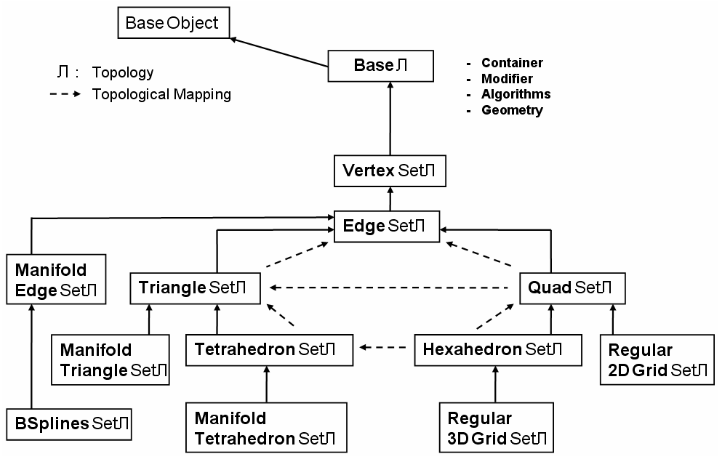
\includegraphics[width=0.85\textwidth]{topology/BW_Topology_Family_Tree.png}
     \caption{Family tree of topology objects. Dashed arrows indicate possible {\em Topological Mappings} from a topology object to another.}
    \label{fig:BW_Topology_Family_Tree}
\end{figure}

Topology objects are composed of four functional members:{\em Container}, {\em Modifier}, {\em Algorithms} and {\em Geometry}.

\begin{itemize}

 \item The {\em Container} member creates and updates when needed two complementary arrays (see Fig.~\ref{fig:BW_Sub_Shell_Diagram}). The former describes the $l$-cells included in a single $k$-cell, $l<k$, while the latter gives the $k$-cells adjacent to a single $l$-cell.
 
 \item The {\em Modifier} member provides low-level methods that implement elementary topological changes such as the removal or addition of an element. 
 
 \item The {\em Algorithms} member provides high-level topological modification methods (cutting, refinement) which decompose complex tasks into low-level ones). 
 
 \item The {\em Geometry} member provides geometrical information about the mesh ({\em e.g.} length, normal, curvature, ...) and requires the knowledge of the vertex positions stored in the {\em Degrees of Freedom} component. 
 
\end{itemize}


\begin{figure}[ht]
    \centering
        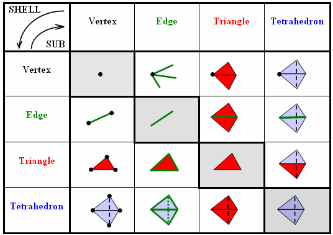
\includegraphics[width=0.6\textwidth]{topology/Sub_Shell_Diagram}
    \caption{The two topological arrays stored in a {\em Container} correspond to the upper and lower triangular entries of this table. The upper entries provide the $k$-cells adjacent to a $l$-cell, $l<k$. The lower entries describe the $l$-cells included in a $k$-cell. Similar table exists for quad and hexahedron elements.}
    \label{fig:BW_Sub_Shell_Diagram}
\end{figure}

\subsection{Component-Related Data Structure}

A key feature of our design is that containers storing mesh information (material stiffness, list of fixed vertices, nodal masses, ...) are stored in {\em components} and spread out in the simulation tree. This modular approach is in sharp contrast with a centralized storage of information in the mesh data structure through the use of generic pointers or template classes.  

Another choice is that most containers are simple arrays with contiguous memory storage and a short direct access time.
This is important for real-time simulation, but bears some drawbacks when elements of these arrays are being removed since it entails the renumbering of elements. For instance, when a single element is removed, the last array element is renumbered such that the array stays contiguous. Fortunately, all renumbering tasks that maintain consistent arrays can be automated and hidden to the user when topological changes in the mesh arise.
Besides, time to update data structures does not depends on the total number of mesh elements but only on the number of modified elements.
Therefore, in our framework, mesh data structures are stored in simple and efficient containers, the complexity of keeping the container consistent with topological changes being automated.

There are as many containers as topological elements: vertices, edges, triangles, ... . These containers are similar to the STL {\em std::vector} classes and allow one to store any component-related data structure. A typical implementation of spring-mass models would use an edge container that stores for each edge, the spring stiffness and damping value, the $i^{th}$ element of that container being implicitly associated with the $i^{th}$ edge of the topology. Finally, two other types of containers may be used when needed. The former stores a data structure for a subset of topological elements (for instance pressure on surface triangles in a tetrahedralisation) while the latter stores only a subset of element indices.


\subsection{Handling Topological Changes}

\noindent 
Surgery simulation involves complex topological changes on meshes, 
for example when cutting a surface along a line segment, or when locally refining a volume before removing some tissue.
However, one can always decompose these complex changes into a sequence of elementary operations, 
such as adding an element, removing an element, renumbering a list of elements or modifying a vertex position.

Our approach to handle topological changes makes the update of data structures transparent to the user, through a mechanism of propagation of topological events.
A topological event corresponds to the intent to add or to
remove a list of topological elements. But the removal of elements cannot be tackled in the same way as the addition of elements. Indeed, the element removal event must be first notified to
the other components before the element is actually removed by the {\em Modifier}.
Conversely, element addition is first processed by the {\em Modifier} and then element addition event is notified to other components (see Fig.~\ref{fig:Order_Notifications}).
Besides, the events notifying the creation of elements also include a list of ancestor elements. Therefore, when splitting one triangle into two sub-triangles (see Fig.~\ref{fig:7_Steps_Cutting_Algorithm}), each component-related information ({\em e.g.} its Young modulus or its mass density) associated with a sub-triangle will be created knowing that the sub-triangle originates from a specific triangle. Such mechanism is important to deal with meshes with non-homogeneous characteristics related to the presence of pathologies.

\begin{figure}[ht]
    \centering
        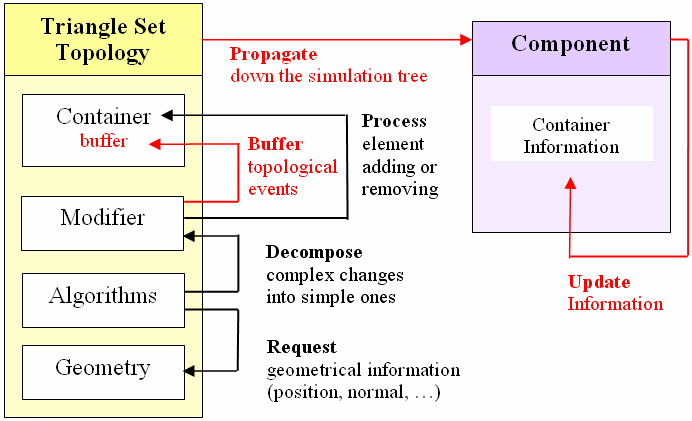
\includegraphics[width=0.7\textwidth]{topology/Handling_Changes}
    \caption{Handling topological changes, with the example of a {\em Triangle Set Topology}. 
    {\em Component} corresponds to any component of the simulation which may need topological information to perform a specific task.
    Black features indicate the effective change process. Red features show the steps of event notification.}
    \label{fig:Handling_Changes}
\end{figure}

\begin{figure}[ht]
 \centering
 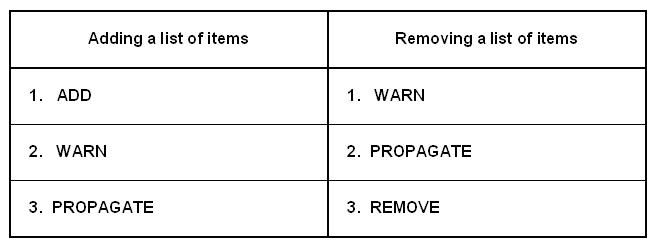
\includegraphics[width=0.65\linewidth]{topology/Order_Notifications}
  \caption{Order to respect when adding or removing an item. WARN means : add the current topological change (add or delete a list of items) in the list of TopologyChanges. PROPAGATE means :  traverse the simulation tree with a TopologyChangeVistor to send the current topological change event to all force fields, constraints, mappings, etc.}
 \label{fig:Order_Notifications}
\end{figure}


\begin{figure}[ht]
    \centering
        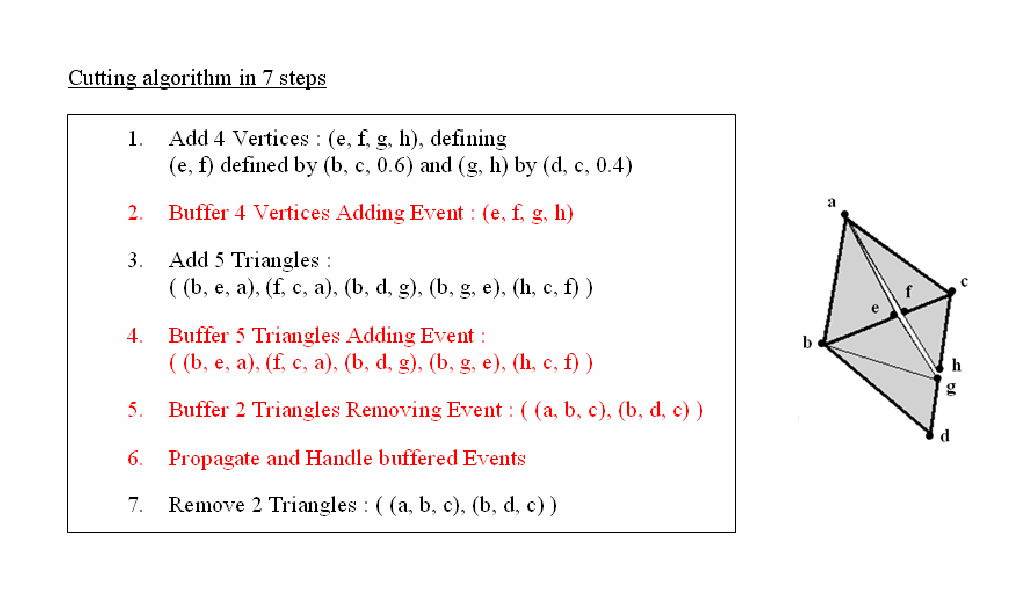
\includegraphics[width=0.8\textwidth]{topology/7_Steps_Cutting_Algorithm}
    \caption{Seven steps to perform cutting along two triangles (these generic steps would be the same to cut an arbitrarily number of triangles).
    Black steps indicate the effective change process. Red steps show the steps of event notification.}
    \label{fig:7_Steps_Cutting_Algorithm}
\end{figure}


The mechanism to handle topological changes is illustrated by Fig.~\ref{fig:Handling_Changes}.
The notification step consists in accumulating the sequence of
topological events  involved in a high-level topological change into a buffer stored in
the {\em Container}. Then the event list is propagated to all its
neighbors and leaves beneath by using a visitor mechanism, called a
{\em Topology Visitor}. Once a given component is visited, the topological
events are actually processed one by one and the data structure used to store mesh related information are automatically updated.

In practice, for each specific component ({\em e.g.} spring-mass mechanical component), a set of callback functions are provided describing how to update the data structure ({\em e.g.} spring stiffness and damping values) when adding or removing an element ({\em e.g.} the edges defined by the two extremities of the springs).
We applied the observer design pattern so that component-related data structures update themselves automatically.


\subsection{Combining Topologies}

Handling a single mesh topology in a surgery simulation scene is often too restrictive. There are at least three common situations where it is necessary to have, for the same mesh, several topological descriptions sharing the same degrees of freedom: the {\em boundary}, {\em composite} and {\em surrogate} cases. In the {\em boundary } scenario,  specific  
algorithms may be applied to the boundary of a mesh, the boundary of tetrahedral mesh being a triangulated mesh and that of a triangular mesh being a polygonal line. For instance, those algorithms may consist of applying additional membrane forces ({\em e.g.} to simulate the effect of the Glisson capsule in the liver) or visualizing a textured surface. Rather than designing specific simulation components to handle triangulations as the border of tetrahedrisations, our  framework allows us to create a triangulation topology object from  a tetrahedrisation mesh and to use regular components associated with triangulations.

The {\em composite} scenario consists in having a mesh that includes several types of elements: triangles with quads, or hexahedra with tetrahedra. Instead of designing specific components for those composite meshes, it is simpler and more versatile to reuse components that are dedicated to each mesh type. Finally the {\em surrogate} scenario corresponds to cases where one topological element may be replaced by a set of elements of a different type with the same degrees of freedom. For instance a quad may be split into two triangles while an hexahedron may be split into several tetrahedra. Thus a quad mesh may also be viewed as a triangular mesh whose topology is constrained by the quad mesh topology.

\begin{figure}[ht]
    \centering
        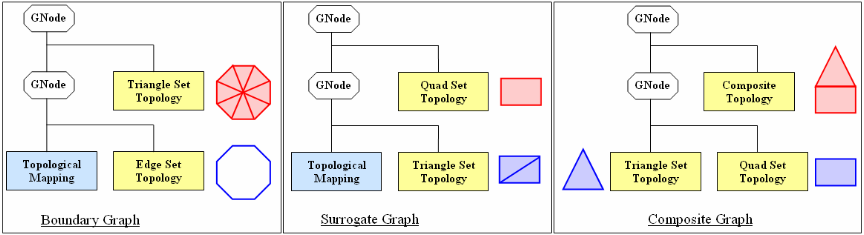
\includegraphics[width=1.0\textwidth]{topology/Combining_Topologies}
    \caption{Three scenari examples to combine topologies. ({\em From left to right}) A {\em Boundary Graph} from a triangle set to an edge set, a {\em Surrogate Graph} from a quad set to an triangle set and a {\em Composite Graph} superseding a quad set and a triangle set.}
    \label{fig:Combining_Topologies}
\end{figure}

These three cases can be handled seamlessly by using a graph of multiple topologies, the topology object being at the top node having the specific role of controlling the topologies below. Although we chose to duplicate topological information in memory, it has no effect on the time required to compute the forces.  Fig.~\ref{fig:Scene_Graph_TopologicalMapping} provides an example of a border scenario (triangulation as the border of a tetrahedralisation) while Fig.~\ref{fig:Combining_Topologies} shows general layout of topology graphs in the three cases described previously. In any cases, those graphs include a dedicated component called a {\em Topological Mapping} whose objectives are twofold. First, they translate topological events originating from the master topology ({\em e.g.} remove this quad) into topological actions suitable for the slave topology ({\em e.g} remove those two triangles for a surrogate scenario). Second, they provide index equivalence  between global numbering of elements in the master topology ({\em e.g} a triangle index in a tetrahedralisation topology ) and local numbering in the slave topology ({\em e.g} the index of the same triangle in the border triangulation). Possible {\em Topological Mappings} from a topology object to another have been represented by blue arrows in Fig.~\ref{fig:BW_Topology_Family_Tree}.

Note that those topology graphs can be combined and cascaded, for instance by constructing the triangulation border of a tetrahedrisation created from an hexahedral mesh.  But only topology algorithms of the master topology may be called to simulate cutting or to locally refine a volume. By combining topology graphs with generic components one can simulate fairly complex simulation scenes where topological changes can be seamlessly applied.


\subsection{An example of Topological Mapping : from TetrahedronSetTopology to TriangleSetTopology}

A TopologicalMapping is a new kind of Mapping which converts an
input topology to an output topology (both topologies are of type
BaseTopology).
\\

It first initializes the mesh of the output topology from the mesh
of the input topology, and it creates the two Index Maps that
maintain the correspondence between the indices of their common
elements.
\\

Then, at each propagation of topological changes, it translates the
topological change events that are propagated from the input
topology into specific actions that call element adding methods or
element removal methods on the output topology, and it updates the
Index Maps.
\\

So, at each time step, the geometrical and adjacency information are
consistent in both topologies.

Here is the scene-graph corresponding to the simulation of an object
which can be represented as a tetrahedral volume (on which one
volume force is applied) or as a triangular surface (on which two
surface forces are applied). Note that the Visual Model and the
Collsion Model are attached to the surface mesh of the object :


\begin{figure}[ht]
 \centering
 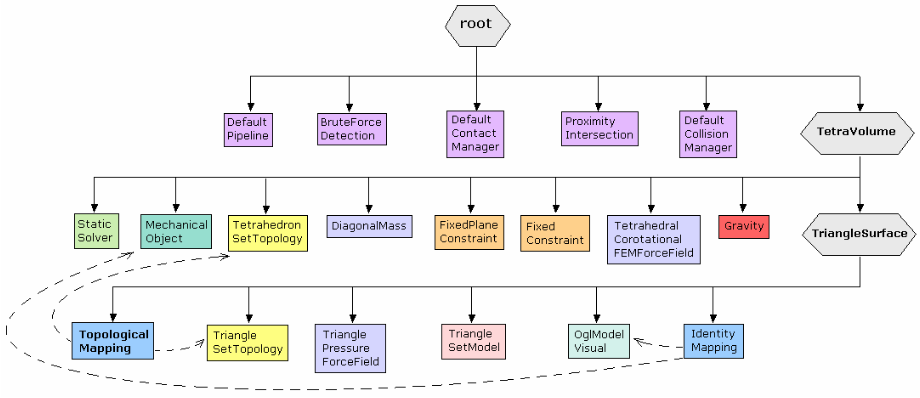
\includegraphics[width=1.0\linewidth]{topology/Scene_Graph_TopologicalMapping}
  \caption{Scene Graph illustrating a TopologicalMapping from a TetrahedronSetTopology to a TriangleSetTopology.}
 \label{fig:Scene_Graph_TopologicalMapping}
\end{figure}

Let us consider an example where the user wants to remove one tetraheron (whose one triangle at least is visible) from the tetrahedral volume.
The component Tetra$2$TriangleSetTopology handles this topological change by following five steps :
\\


\begin{itemize}

    \item \textbf{Step $1$.} The user right-clicks on visible triangle T in the scene, which is detected by the Collision Model and indexed by $loc\_T$ in the triangular surface mesh.
    
\begin{figure*}
 \centering
 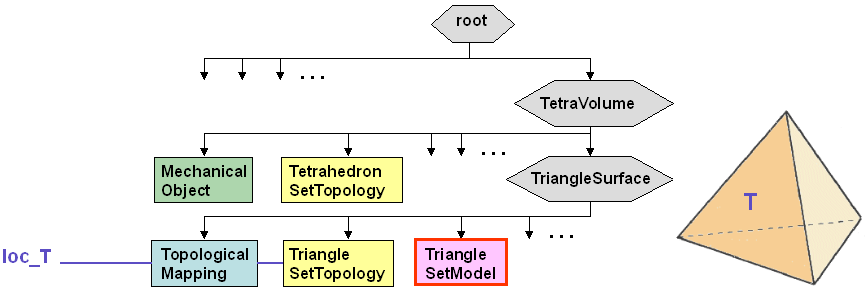
\includegraphics[width=1.0\linewidth]{topology/TopoMap_example_1}
  \caption{Scenario when the user wants to remove one tetraheron.- Step 1.}
 \label{fig:TopoMap_example_1}
\end{figure*}


    \item \textbf{Step $2$.} If a Topological Mapping of type ( input = TetrahedronSetTopology, output = TriangleSetTopology ) does exist, the index map $Loc2GlobVec$ is requested to give the index $glob\_T$ which is indexing the triangle T in the tetrahedral volume mesh. 
The TetrahedraAroundTriangle gives then the index $ind\_TE$ which is indexing the unique tetrahedron TE containing T. 
We call the action RemoveTetrahedra($< ind\_TE >$) on the input topology.

\begin{figure*}
 \centering
 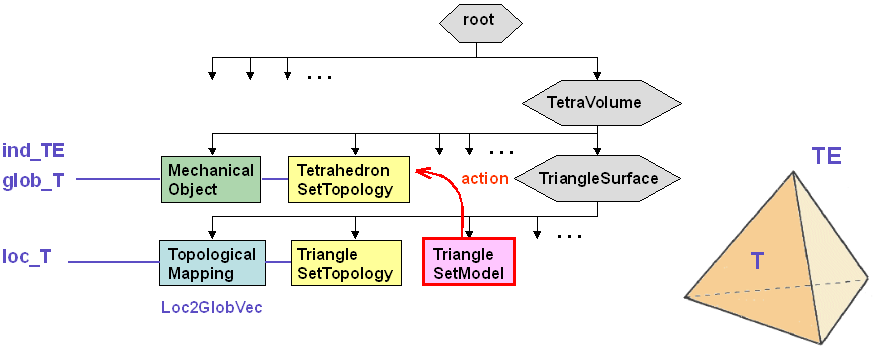
\includegraphics[width=1.0\linewidth]{topology/TopoMap_example_2}
  \caption{Scenario when the user wants to remove one tetraheron.- Step 2.}
 \label{fig:TopoMap_example_2}
\end{figure*}


    \item \textbf{Step $3$}. The TetrahedronSetTopology notifies all the removal events, that are successively concerning one tetrahedron, one or more isolated triangles, the possibly isolated edges and the possibly isolated points.

\begin{figure*}
 \centering
 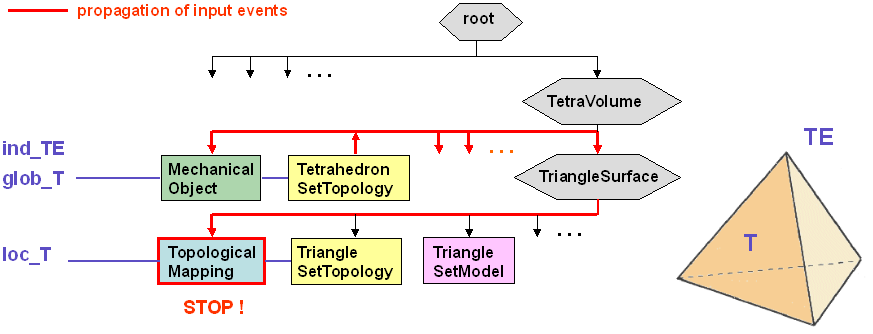
\includegraphics[width=1.0\linewidth]{topology/TopoMap_example_3}
  \caption{Scenario when the user wants to remove one tetraheron.- Step 3.}
 \label{fig:TopoMap_example_3}
\end{figure*}


    \item \textbf{Step $4$.} The propagation of topological events reaches a Topological Mapping which is strictly lower in the scene graph, then it stops.
The Tetra2TriangleTopologicalMapping translates the input events into output actions on the TriangleSetTopology.
The event Tetrahedron removal is translated into the action AddTriangles ( $<$ indices of new visible triangles $>$ ).
The event Triangle removal is translated into the action RemoveTriangles ( $<$ indices of destroyed triangles $>$, removeDOF $=$ false ), where (removeDOF $=$ false) indicates that the DOFs of the isolated points must not be deleted because they have already been removed by the input topology.
The Index maps ( Loc2GlobVec, Glob2LocMap, In2OutMap ) are requested and updated to maintain the correspondence between the items indices in input and output topologies.

\begin{figure*}
 \centering
 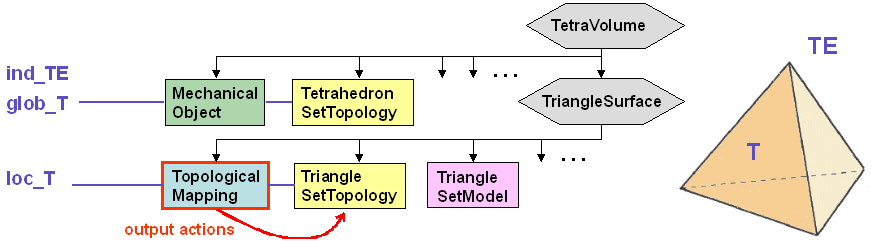
\includegraphics[width=1.0\linewidth]{topology/TopoMap_example_4}
  \caption{Scenario when the user wants to remove one tetraheron.- Step 4.}
 \label{fig:TopoMap_example_4}
\end{figure*}


    \item \textbf{Step $5$.} The adding events concerning one or more new visible triangles and the removal events concerning one or more isolated triangles are notified from the TriangleSetTopology.

\begin{figure*}
 \centering
 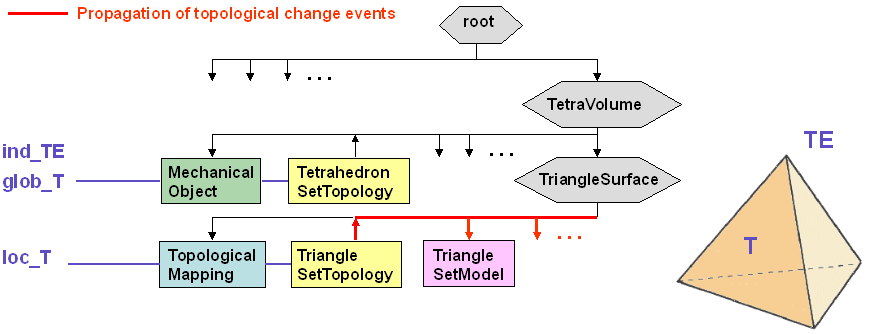
\includegraphics[width=1.0\linewidth]{topology/TopoMap_example_5}
  \caption{Scenario when the user wants to remove one tetraheron.- Step 5.}
 \label{fig:TopoMap_example_5}
\end{figure*}

\end{itemize}

\subsection{Example of scene file with a topological mapping}

\begin{figure*}
 \centering
 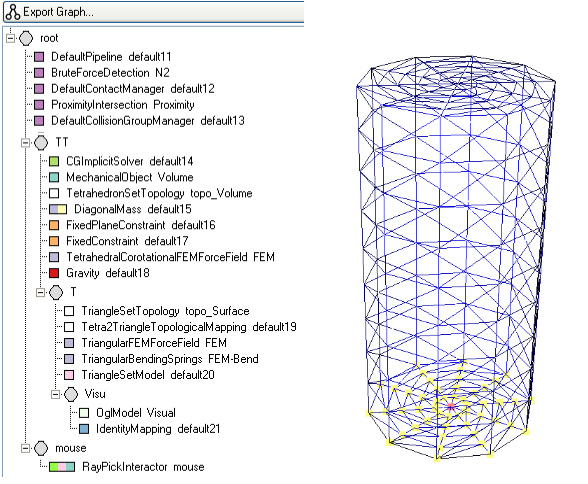
\includegraphics[width=0.9\linewidth]{topology/cylinder_example}
  \caption{Scene Graph simulating a bending cylinder as a tetrahedral volume and as a triangular surface (the cylinder membrane)}
 \label{fig:cylinder_example}
\end{figure*}

\newpage

Here is the scene file corresponding to the example :

\begin{verbatim}

<Node name="root" dt="0.05" showBehaviorModels="1" showCollisionModels="0" showMappings="0" 
 showForceFields="0" showBoundingTree="0" gravity="0 0 0">
  
	<Object type="CollisionPipeline" verbose="0" />
	<Object type="BruteForceDetection" name="N2" />
	<Object type="CollisionResponse" response="default" />
	<Object type="MinProximityIntersection" name="Proximity" alarmDistance="0.8" 
	 contactDistance="0.5" />
	
	<Object type="CollisionGroup" />

	<Node name="TT">
	
		<Object type="EulerImplicit" name="cg_odesolver" printLog="false"/>
		<Object type="CGLinearSolver" iterations="25" name="linear solver" tolerance="1.0e-9" 
		 threshold="1.0e-9" />
		
		<Object type="MeshLoader" name="meshLoader" filename="mesh/cylinder.msh" />
		<Object type="MechanicalObject" name="Volume" />
		<include href="Objects/TetrahedronSetTopology.xml" />

    <Object type="DiagonalMass" massDensity="0.5" />
		<Object type="FixedPlaneConstraint" direction="0 0 1" dmin="-0.1" dmax="0.1"/>
		<Object type="FixedConstraint" indices="0" />		
    <Object type="TetrahedralCorotationalFEMForceField" name="FEM" youngModulus="60" 
     poissonRatio="0.3" method="large" />
    
    <Object type="Gravity" gravity="0 0 0"/>

		<Node name="T">
		
			<include href="Objects/TriangleSetTopology.xml" />
			<Object type="Tetra2TriangleTopologicalMapping" object1="../../Container" object2="Container"/>

      <Object type="TriangularFEMForceField" name="FEM" youngModulus="10" poissonRatio="0.3" 
       method="large" /> 
			
			<Object type="TriangularBendingSprings" name="FEM-Bend" stiffness="300" damping="1.0"/>		
			    
			<Object type="TriangleSet"/>

			<Node name="Visu">
			
				<Object type="OglModel" name="Visual" color="blue" />
				<Object type="IdentityMapping" object1="../../../Volume" object2="Visual" />
				
			</Node>						
			
		</Node>
		
	</Node>
	
</Node>

\end{verbatim}

Here is the example of the included TriangleSetTopology.xml file, where the four members of the {\em TriangleSetTopology} are defined :

\begin{verbatim}

<Node name="Group"> 
  <Object type="TriangleSetTopologyContainer"  name="Container" />
  <Object type="TriangleSetTopologyModifier"   name="Modifier" />
  <Object type="TriangleSetTopologyAlgorithms" name="TopoAlgo"   template="Vec3d" />
  <Object type="TriangleSetGeometryAlgorithms" name="GeomAlgo"   template="Vec3d" />
</Node>

\end{verbatim}

\subsection{How to make a component aware of topological changes ?}

%%%

There are actually a few generic lines of code to add in a component for it to handle topological changes.
\\

If the component is based on topological elements like edges, the main idea is to introduce an object {\em edgeinfo} of type {\em EdgeData} 
and to template it by a data structure {\em EdgeInformation} that is attached to each edge (this data structure has to be defined by the component, to which it is specific).
By calling the method {\em handleTopologyEvents} on the object {\em edgeinfo} (of type {\em EdgeData} $<${\em EdgeInformation}$>$), the component-related data structure is automatically updated (code has been implemented in file {\em EdgeData.inl}).
\\

Here : {\em edgeinfo}$[i]$ is the data structure attached to the edge indexed by $i$ in the topological component {\em EdgeSetTopology}.
\\

In SOFA, among the existing ForceField component able to handle topological changes there are for example : {\em BeamFEMForceField} (for the simple case) and {\em TriangularBendingSprings} (for the complicated case : data structure attached to each edge need to contain indices of points, which must also be updated by the method {\em handleTopologyChange}).
\\

For the simple case, here is how to adapt a Force Field component called {\em totoForceField} (for instance based on elements of type edge) to topological changes : 

\subsubsection{Modifications in header file {\em totoForceField.h} :}

\begin{itemize}

	\item Include the following header :  \begin{verbatim} #include <sofa/component/topology/EdgeData.h> \end{verbatim}
	
	\item Define a structure {\em EdgeInformation} which describes the information attached to each edge (for example {\em spring stiffness},
{\em spring length}, ...)
	
	\item Add an object {\em edgeinfo} of type {\em EdgeData} templated by the type
{\em EdgeInformation} : \begin{verbatim} topology::EdgeData<EdgeInformation> edgeinfo;  \end{verbatim}

	\item Declare the virtual method {\em handleTopologyChange} : \begin{verbatim} virtual void handleTopologyChange(); \end{verbatim}

  \item Add the callback function for the creation of edges :

\begin{verbatim} 

static void EdgeCreationFunction(
    int edgeIndex,
    void* param,
    EdgeInformation &ei,
    const topology::Edge& ,
    const sofa::helper::vector< unsigned int > &,
    const sofa::helper::vector< double >&
);


\end{verbatim} 

\end{itemize}

\subsubsection{Modifications in inline file {\em totoForceField.inl} :}


\begin{itemize}

	\item Add at the end of the method {\em init()} to specify the callbacks :
	
	\begin{verbatim} 

edgeinfo.setCreateFunction(EdgeCreationFunction);
edgeinfo.setCreateParameter( (void *) this );
edgeinfo.setDestroyParameter( (void *) this );

\end{verbatim} 
	
	\item Implement the method {\em handleTopologyChange()} :
	
  \begin{verbatim} 

template <class DataTypes>
void totoForceField<DataTypes>::handleTopologyChange()
{

    std::list< const sofa::core::componentmodel::topology::TopologyChange* >
::const_iterator itBegin = _topology->firstChange();

    std::list< const sofa::core::componentmodel::topology::TopologyChange*>
::const_iterator itEnd = _topology->lastChange();

    edgeinfo.handleTopologyEvents(itBegin,itEnd);
    
}
\end{verbatim} 

	\item Implement the method {\em EdgeCreationFunction} (usefull for the initialization of the data attacheed to a new edge) :
	
	\begin{verbatim} 
	
template<class DataTypes>
void totoForceField<DataTypes>::EdgeCreationFunction(

int edgeIndex, void* param, EdgeInformation &ei,
const topology::Edge& e,  const sofa::helper::vector< unsigned int > &a,
const sofa::helper::vector< double >&
)

{

    totoForceField<DataTypes> *ff= (totoForceField<DataTypes> *)param;

    if (ff) {

      ei.champ = value; // initialiser tous les champs de "edgeinfo[i]"

      (...)

    }
}
	
	\end{verbatim} 
	
	
\end{itemize}

At any time, it is possible to access the information from the container member of the topology (so as to get some neighborhood information) by using a pointer to the {\em BaseMeshTopology} API :

	\begin{verbatim} 
	
sofa::core::componentmodel::topology::BaseMeshTopology* _topology;
_topology = getContext()->getMeshTopology();

	\end{verbatim} 


\subsection{What happens when I split an Edge ?}

\begin{figure*}[htpb]
 \centering
 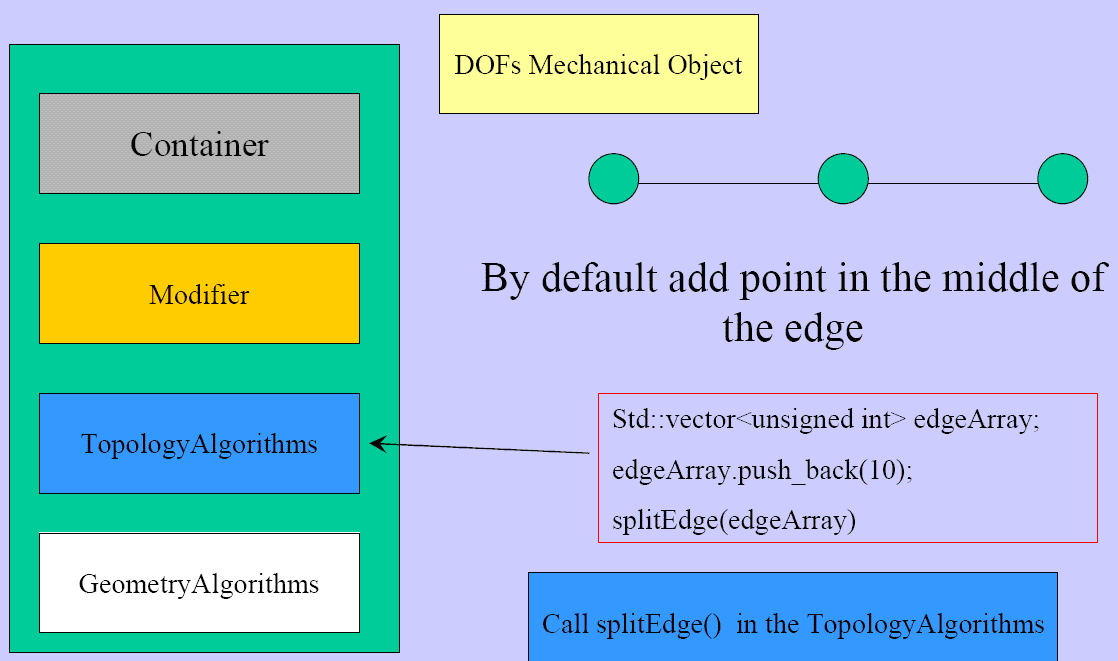
\includegraphics[width=0.9\linewidth]{topology/Topology_Example_1}
 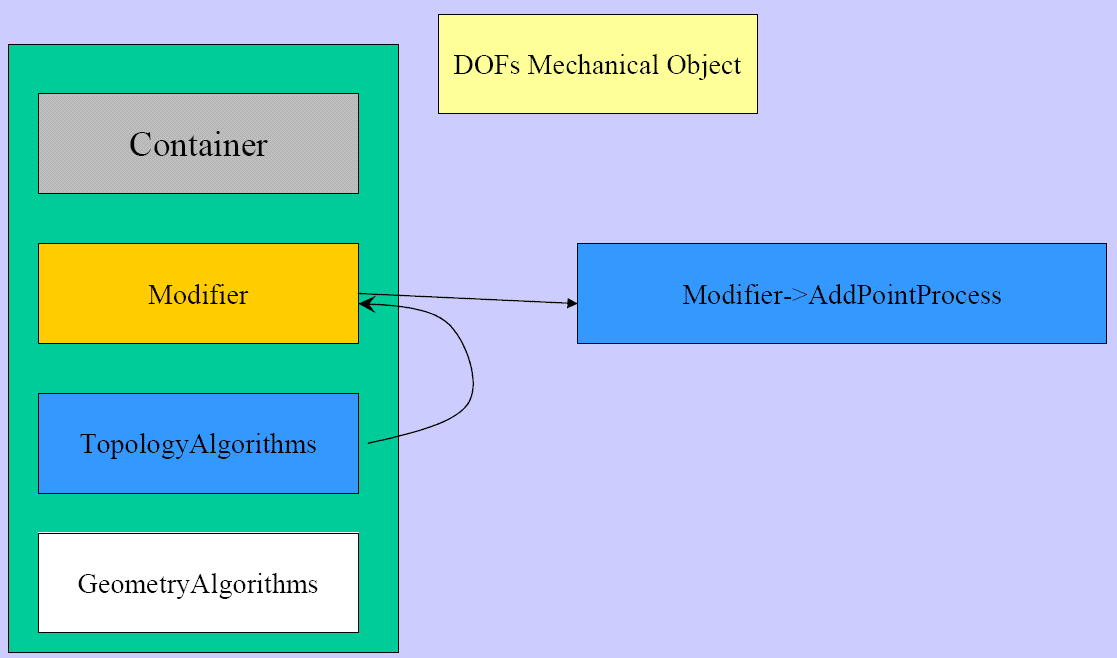
\includegraphics[width=0.9\linewidth]{topology/Topology_Example_2}
  \caption{What happens when I split an Edge ? - Step 1. 2.}
 \label{fig:Topology_Example_12}
\end{figure*}

\newpage

\begin{figure*}[htpb]
 \centering
 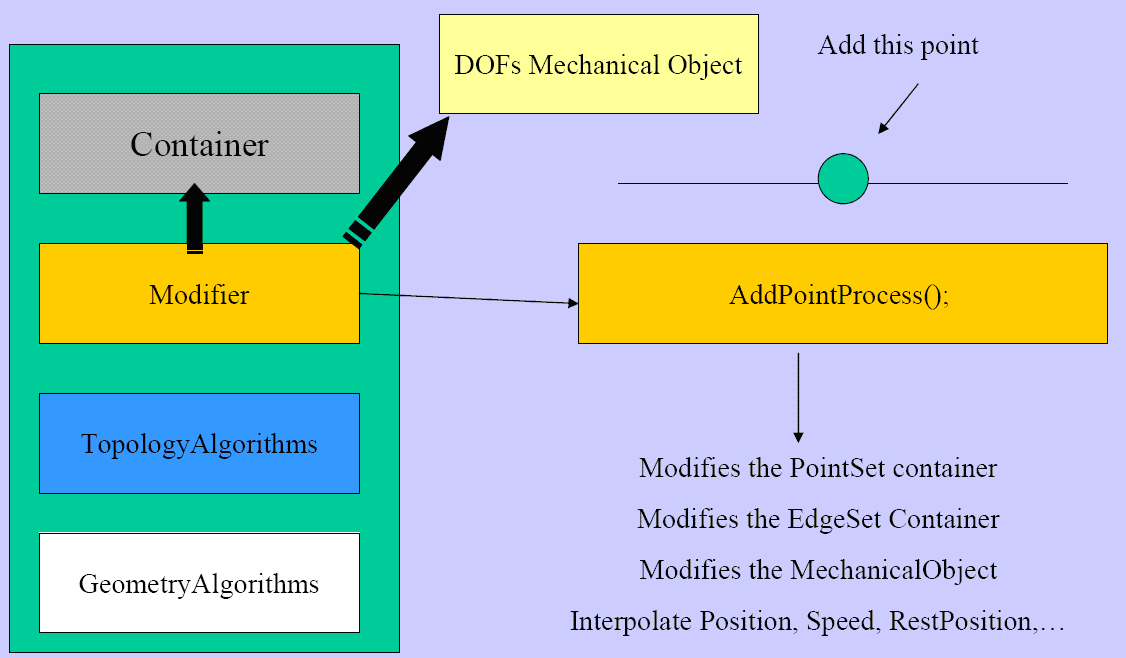
\includegraphics[width=0.9\linewidth]{topology/Topology_Example_3}
 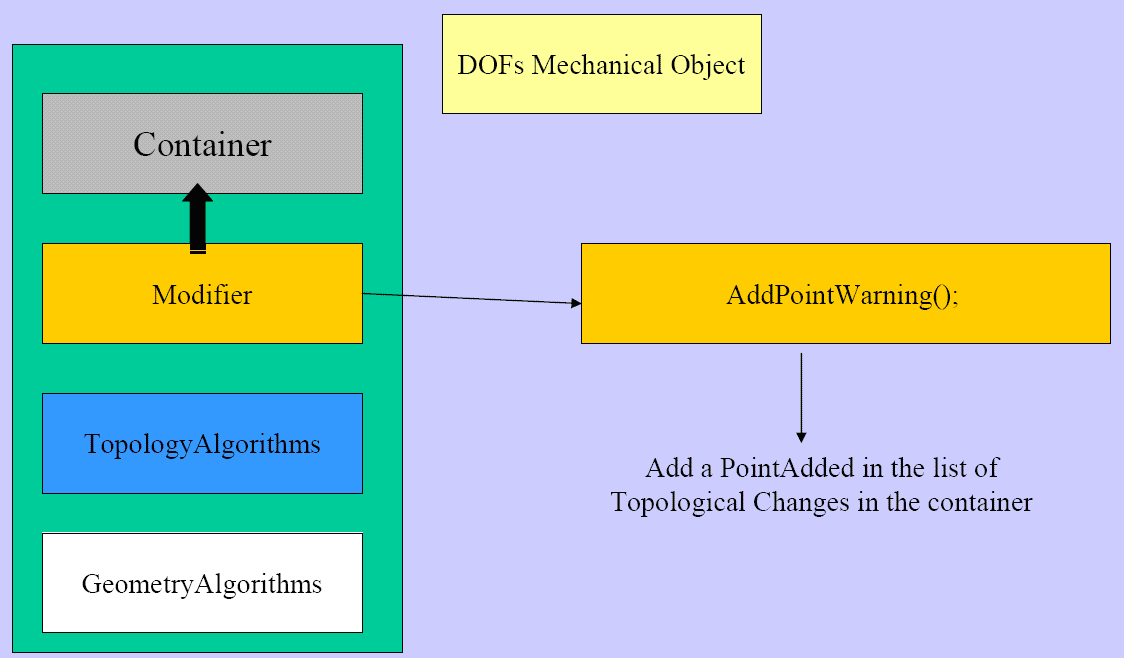
\includegraphics[width=0.9\linewidth]{topology/Topology_Example_4}
  \caption{What happens when I split an Edge ? - Step 3. 4.}
 \label{fig:Topology_Example_34}
\end{figure*}

\newpage

\begin{figure*}[htpb]
 \centering
 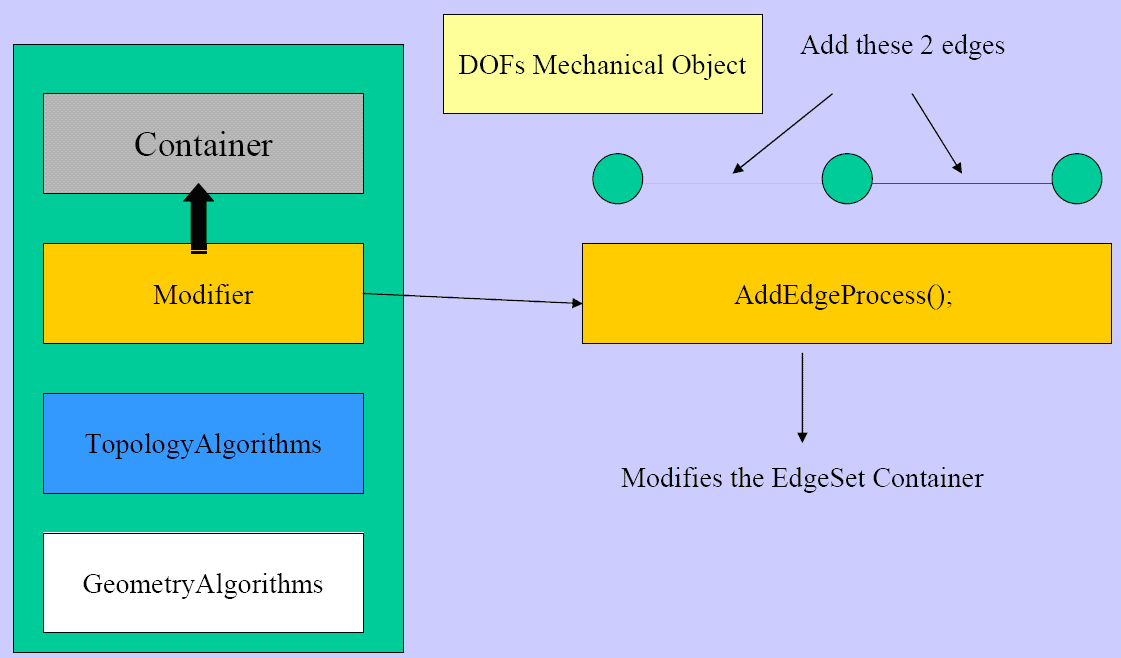
\includegraphics[width=0.9\linewidth]{topology/Topology_Example_5}
 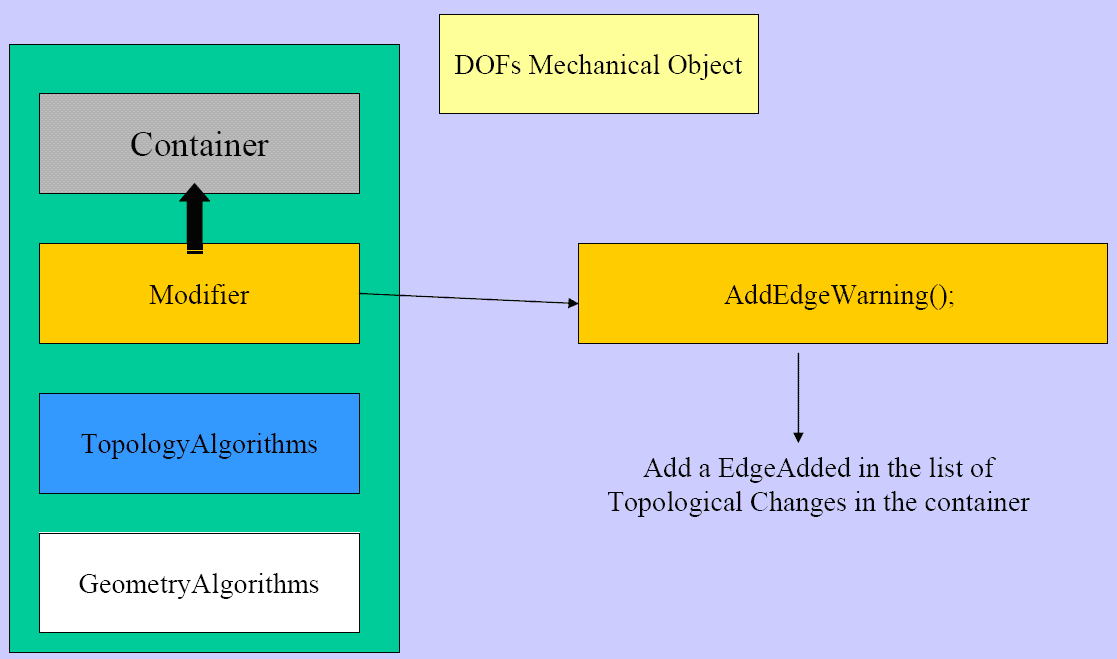
\includegraphics[width=0.9\linewidth]{topology/Topology_Example_6}
  \caption{What happens when I split an Edge ? - Step 5. 6.}
 \label{fig:Topology_Example_56}
\end{figure*}

\newpage

\begin{figure*}[htpb]
 \centering
 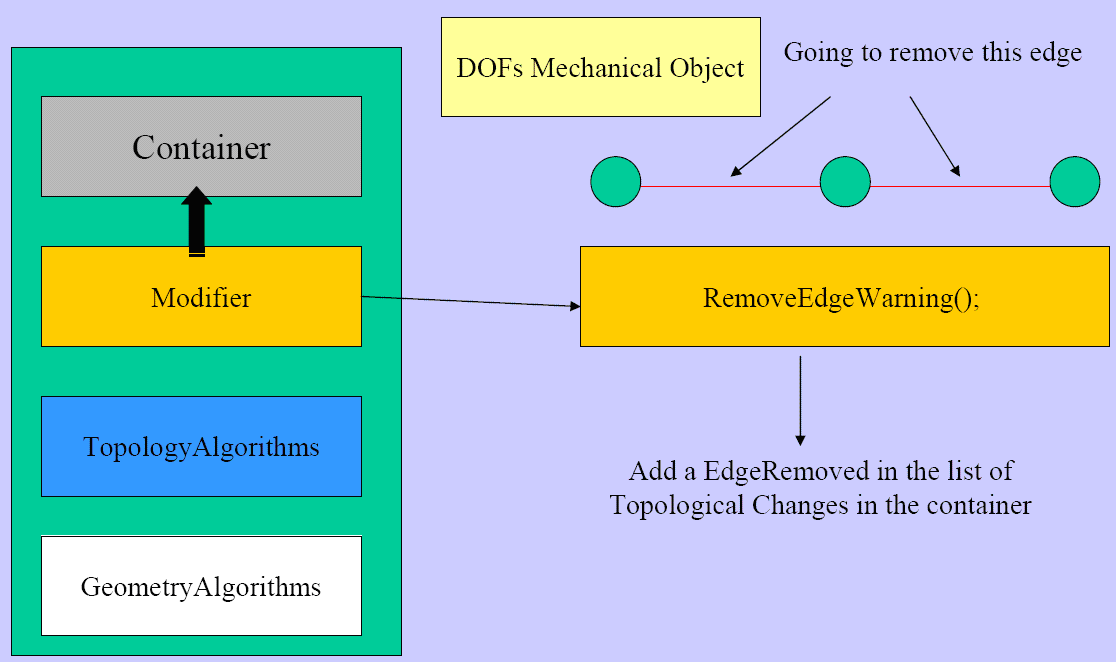
\includegraphics[width=0.9\linewidth]{topology/Topology_Example_7}
 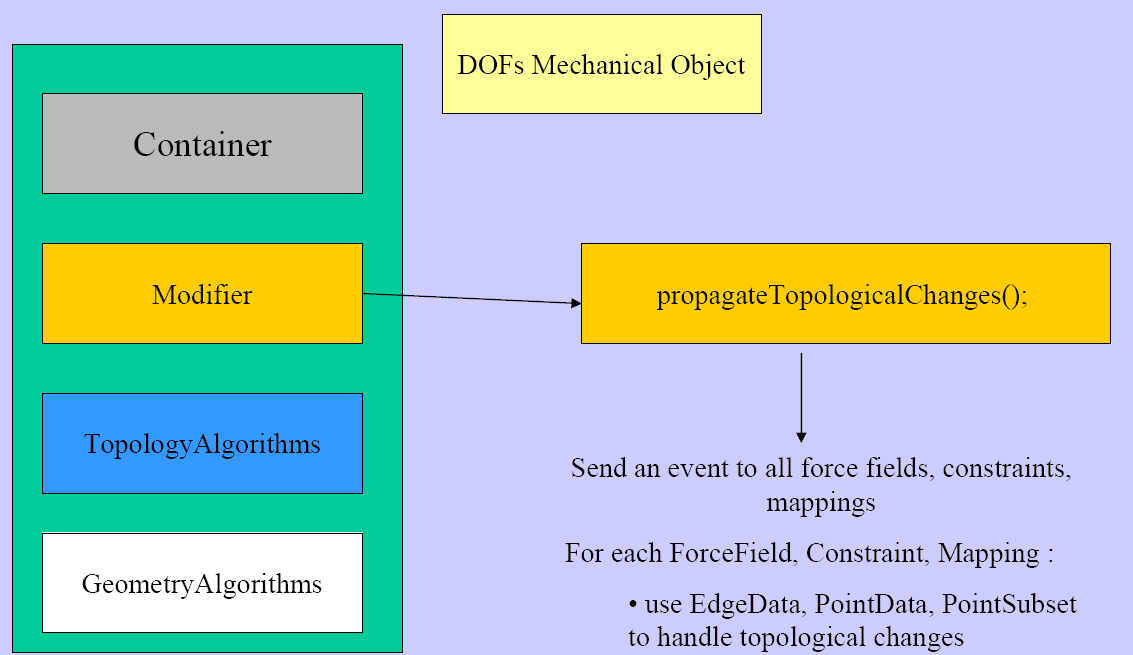
\includegraphics[width=0.9\linewidth]{topology/Topology_Example_8}
  \caption{What happens when I split an Edge ? - Step 7. 8.}
 \label{fig:Topology_Example_78}
\end{figure*}

\newpage

\begin{figure*}[htpb]
 \centering
 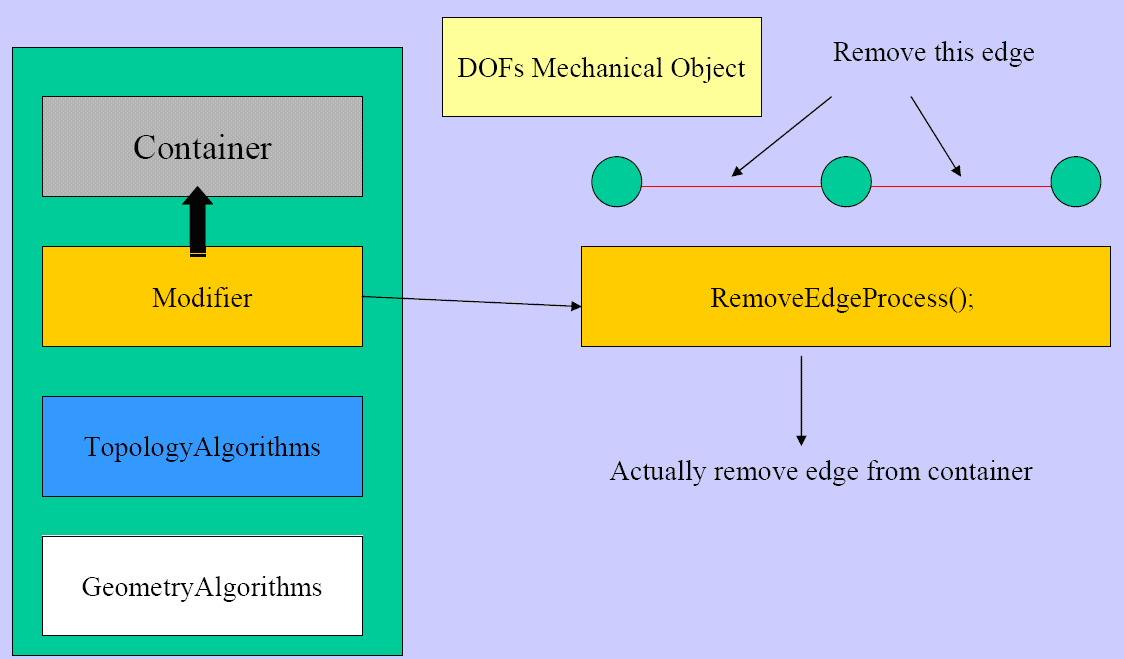
\includegraphics[width=0.9\linewidth]{topology/Topology_Example_9}
  \caption{What happens when I split an Edge ? - Step 9.}
 \label{fig:Topology_Example_9}
\end{figure*}

               
% \subsubsection{Use Cases}
